\chapter{Local maladaptation reduces expansion load during range expansion}
\label{chap:expansionload}

%%\section{Abstract}

%%The biotic and abiotic factors that facilitate or hinder species range expansions are many and complex. We examine the impact of two genetic processes and their interaction on fitness at expanding range edges: local maladaptation resulting from the presence of an environmental gradient, and expansion load resulting from increased genetic drift at the range edge. Results from spatially explicit simulations indicate that the presence of an environmental gradient during range expansion reduces expansion load; conversely, increasing expansion load allows only locally adapted populations to persist (\color{red} OR eliminates maladaptive diversity ? \color{black}) at the range edge. %Increased expansion load reduces maladaptation by necessitating higher local adaptation in order for absolute fitness of a population to be at a sustainable level. 
%%Increased maladaptation reduces the speed of range expansion, leading to increased evolutionary rescue and the reduction of expansion load at the range edge. These results may have ramifications for species being forced to shift their ranges due to climate change or other anthropogenic changes. If rapidly changing climate leads to faster expansion from populations tracking their shifting climatic optimum, populations may suffer increased expansion load beyond previous expectations.

%%\newpage{}


\section{Introduction}

%broad intro:
Species range expansion is a complex process that is widely studied in evolutionary biology, ecology, and conservation biology \citep{Chen:2011, Colautti:2013, Hastings:2005, Phillips:2006, Excoffier:2009, Hallatschek:2010}. An array of ecological and evolutionary factors are known to affect the success or failure of range expansion, such as dispersal limitation \citep{Hargreaves:2014b, Marsico:2009, Hastings:2005}, interspecific competition \citep{Case:2000, Price:2009,Svenning:2014, Louthan:2015}, or an inability to adapt to new conditions \citep{Polechova:2015, Holt:2011, Angert:2008}. A recently growing field of research has focused on an additional effect: the genetic load accumulated during the expansion process \citep{Excoffier:2009, Hallatschek:2010, Peischl:2013, Peischl:2015, Peischl:2015b}. In particular, the increasing frequency of deleterious variants in human populations that have expanded out of Africa have been widely studied \citep{Henn:2015, Do:2015, Lohmueller:2008}. A further process that can increase genetic load during range expansion is maladaptation to the local environment due to gene flow from foreign environments, known as migration load \citep{Kirkpatrick:1997, Barton:2001, Polechova:2015}. In this study, we explore the impacts and interactions of heterogeneous selection due to an environmental gradient and the accumulation of deleterious mutations during range expansion.

% range expansions:
During range expansions, an intriguing suite of population genetic processes can change the course of evolution compared to populations that are growing in size without movement. Populations at the expanding front of a species range undergo serial founder events where each new colonization into further territory creates a population bottleneck, leading to reduced genetic diversity in what becomes the new edge population and the primary source of future colonists. These processes create a persistently reduced effective population size at the range edge, decreasing the efficacy of selection and increasing the strength of random genetic drift. This leads to the process of allele surfing \citep{Klopfstein:2006}, whereby a deleterious mutation that arises at the range edge is more likely to drift to high frequency than it otherwise would if it arose in the denser core of the species range. Because selection is ineffective, strongly deleterious alleles may persist and reach higher frequencies than expected in a population at equilibrium \citep{Peischl:2015}. Theoretical work shows that allele surfing is the main cause of increased deleterious allele frequency within recently expanded populations \citep{Excoffier:2009}. The reduction in fitness due to the accumulation of these deleterious alleles is termed expansion load \citep{Peischl:2013,Peischl:2015}.

% deleterious mutations:
Empirical evidence also supports the predictions of both higher frequency and increased effect sizes of deleterious mutations in recently expanded populations. Expansion load has been posited as an explanation for the accumulation of deleterious alleles in human populations that have undergone recent geographic expansions \citep{Karlsson:2014}, e.g. genetic diseases in populations of Quebec \citep{Scriver:2001, Yotova:2005, Labuda:1997} and Scandinavia \citep{Norio:2003}%check that this ref is appropriate
. A large point of controversy, however, is the likelihood of these deleterious mutations persisting at high frequencies in modern populations. As human expansion out of Africa proceeded, deleterious mutations of larger effect rose in frequency, shifting the entire distribution of allelic effect sizes upwards through time \citep{Henn:2015}. Expansion load may thus have serious repercussions in many other species that undergo expansions, such as those recolonizing formerly glaciated areas \citep{Hewitt:1999}, colonizing a new continent \citep{Sakai:2001}, or tracking recent climate change \citep{Chen:2011}. Understanding the detriment caused by this process may aid in efforts to combat invasive species or in assisted migration. As global climate change proceeds, more species than ever may be required to move their ranges in order to survive, and if fitness losses simply due to the expansion process are common, populations may be left at higher risk for extinction from stochastic, catastrophic events. 

% environmental gradients:
A second evolutionary process that can affect range expansion is local adaptation to heterogeneous environmental conditions. Selective environments can vary over space: e.g. environmental gradients for temperature or photoperiod from equatorial to polar latitudes influence important traits \citep{Conover:1992, Montague:2008}. A foundational study by \citet{Kirkpatrick:1997} showed that steep environmental gradients can impede range expansion due to the migration of individuals from the range core to the range edge preventing local adaptation to edge conditions. Central populations existing on an environmental gradient receive symmetric migration from populations both higher and lower on the gradient, leaving the population mean unchanged. In contrast, at a range edge, migration is asymmetric and proportionally larger from core populations into small edge populations, causing edge populations to be swamped by locally maladaptive alleles and diverge from their local optimum. Therefore, when migration rates are high enough, the edge population can fail to adapt. When the environmental gradient is steep enough, the edge populations can experience sufficient fitness reductions to result in local extinction and prevent range expansion. Further studies \citep{Barton:2001, Polechova:2015} have added additional biological realism to models of range expansion (including evolution of genetic variance and effects of genetic drift), confirming theoretically that evolutionary processes alone can form a stable range edge. 


% their interaction and what this study is doing:
It is clear that expansion load can result in reduced fitness of recently expanded populations, and that heterogeneous selection along an environmental gradient can result in local maladaptation of populations at the edge of a species range. These two evolutionary processes -- maladaptation from underlying environmental gradients and expansion load from surfing of deleterious mutations at range edges -- may occur simultaneously in many range expansions and could interact in interesting ways that have not previously been studied. We consider two contrasting \emph{a priori} hypotheses for how they may interact. One possibility is that local maladaptation and expansion load may interact positively(i.e., each making the effects of the other more pronounced). This may be expected because both processes could lead to smaller population sizes at the expanding front, and both are stronger with greater genetic drift: expansion load increases because greater drift would cause more deleterious alleles to increase in frequency, and maladaptation worsens because greater drift would eliminate more of the genetic variance needed to respond to local selection. Alternatively, expansion load and local maladaptation could negatively interact, with each partially ameliorating the effects of the other. This is plausible because both forms of load could reduce the pace at which ranges expand, by reducing the fitness of individuals at the range margin. Slower expansion enables fitter alleles to reach the edge through migration and to rescue populations suffering from accumulated expansion load. Similarly, slower range expansion could allow more time for populations to adapt to local conditions.

We investigate these alternative hypotheses to establish the role of expansion load and migration load in isolation as well as in combination. Our goal is to employ the most biologically reasonable parameters possible within the realm of our model. Using individual-based simulations on a two-dimensional, spatially explicit, and approximately continuous landscape, we compare the reductions in fitness (load) that populations experience during range expansions over a series of environmental gradients and deleterious mutation rates. These results have implications for the predicted prevalence of expansion load in species across various types of environments and inform our understanding of the complex demographic and genetic processes that occur during range expansions. 


\section{Methods}


% broad summary of what we modeled:
We model a species range expansion forward in time using the simulation program \textsc{nemo} \citep{Guillaume:2006}. The population undergoes an initial burn-in period to mutation-selection equilibrium, after which it is allowed to expand across an empty landscape. Individuals are monoecious and diploid, possessing both a quantitative trait experiencing stabilizing selection and a set of loci subject to unconditionally deleterious mutations. We compare three environmental gradients over which expansion occurs, and three genome-wide deleterious mutation rates. All combinations of parameter values are listed in Table \ref{tab:paramresults}. We ran twenty independent replicates for each of our simulated scenarios.


\subsection*{The Model}

% landscapes
The environmental gradient underlying the landscape changes in only one dimension, along the axis of expansion. We compare three values for the steepness of this gradient, $b$, which defines the change in phenotypic optimum over space: a flat landscape with no gradient ($b = 0.0$), a shallow gradient ($b = 0.0375$), and a steep gradient ($b = 0.375$). On the shallow gradient, an average dispersal distance of an individual would result in a fitness loss of $0.5\%$ if it were perfectly adapted in its natal environment, whereas on the steep gradient, an average dispersal event would reduce an individual's fitness by $5\%$ given perfect adaptation in its natal environment. Each of these gradients results in a different equilibrium level of migration load in populations.

% landscape and population details - and general model details
We model space explicitly on a $2000\times40$ unit landscape using a modified version of \textsc{nemo} available at \url{https://github.com/kjgilbert/NemoDispersalKernel}. Each $1\times40$ unit slice of the landscape is referred to as a cross-section (Figure \ref{fig:landscape}). This modification allows a discrete approximation of continuous space. The landscape is divided into 80,000 $1\times1$ square units, which we call cells. The dispersal kernel and breeding window occur across cells, allowing individuals to interact over a larger spatial scale.  Lifecycle events occur in the order of breeding, dispersal, selection, and then population regulation. Subpopulation regulation enforces a carrying capacity of 6 individuals per cell, but because breeding is not limited to within one cell, the realized neighborhood size as defined by \citet{Wright:1946} is approximately 300 individuals.

%--------- Remi's calculations ---------
%Here is how I calculated it. Note that I used the original formal definition by Wright but in empirical papers, authors seem to playfully use different definitions!
%The "neighbourhood size" is the number of individuals present in the "neighbourhood area", an area where parents can be considered representative of the offspring. The first one to use this term was Wright. In Wright 1945 (page 41). Wright defines the "neighbourhood area" as the circle of $2 \sigma$ of radius, where $\sigma$ is the standard deviation of the migration distance. The "neighbourhood size", is therefore $\pi * n$, where $n$ is the number of individuals in a big square of $2 \sigma$ on a side. 
%In our case $\sigma = 2$ demes for both the leptokurtic and normal distribution and the population per small deme is 6. As a a consequence $n = (2*2)^2 * 6 = 96$ and the "neighbourhood size" is $96 * pi \approx 301.59$ individuals.
%------ End of Remi's calculations ------

Populations were initiated at carrying capacity in the left-most $40$ cross-sections of the landscape, which we term the landscape core (Figure \ref{fig:landscape}). After a burn-in period of 15,000 generations, the remaining $1960$ cross-sections of the landscape become available, allowing for expansion to occur. The environmental optimum is constant across any given cross-section.

\begin{figure}[h]
\centering
\makebox[\textwidth]{
        \includegraphics[width=1\linewidth]{Figures/Landscape_Graphic.pdf}}
\caption[~- Landscape graphic.]{Landscape graphic representing an example of the landscape simulated with a grid of units where the burn-in period occurs in the landscape core at the left, expansion proceeds to the right, and any vertical column of units is a cross-section. Actual landscapes were $2000\times40$ units with a $40\times40$ core.}
\label{fig:landscape}
\end{figure}


% breeding
\subsubsection*{Breeding}
Our modified version of \textsc{nemo} creates a breeding window within which individuals may search for a mate within their own cell on the landscape or in nearby cells. Mating probability follows an approximate bivariate Gaussian function which we derive by integrating the probability over each cell within the breeding window. We define the size of this breeding window with the parameter $\sigma_{breed}$, where $f(x,y) \propto \exp{[-(\frac{\Delta x^2}{2\sigma_{breed}^2}+\frac{\Delta y^2}{2\sigma_{breed}^2})]}$ gives the distance traveled to search for a mate in each dimension of the landscape. $\sigma_{breed}$ was held constant at $0.5$ landscape units. The maximum searchable distance was restricted to $4\sigma_{breed}$ with probabilities renormalized to correct for this truncation. This results in a two-dimensional breeding window where an individual's focal cell is the most likely source of a mate and the 12 surrounding cells could be searched for a mate with decreasing probability. This breeding kernel describes the relative probability of each individual within the possible breeding window being chosen as the male parent for a given offspring. When no other individuals are present within the breeding window, an individual self-fertilizes. This will most often happen at the expanding range edge where population densities are lowest and mimics the ability of many plant species to self under conditions of pollen limitation \citep{Hargreaves:2014}. Each female's fecundity was drawn from a Poisson distribution with mean 7 to determine the number of mating events. 

\subsubsection*{Dispersal}
% dispersal
We modeled dispersal for most simulations according to an approximate bivariate Gaussian kernel, similarly to the breeding kernel: $f(x,y) \propto \exp{[-(\frac{\Delta x^2}{2\sigma_{disperse}^2}+\frac{\Delta y^2}{2\sigma_{disperse}^2})]}$. The dispersal kernel gives the forward (in time) migration probabilities for offspring to disperse to a given patch. The maximum dispersal distance was capped at $8\sigma_{disperse}$ units. $\sigma_{disperse}$ for the Gaussian dispersal kernel was set to equal two landscape units. We also simulated a leptokurtic kernel, to test the effects of rare, long-distance dispersal events. The leptokurtic dispersal kernel was a mixture distribution created from a weighted sum of two different Gaussian kernels \citep{Ibrahim:1996} with the same average dispersal distance as the Gaussian kernel and a total kurtosis of 10. This value of kurtosis is not unrealistic for long-distance dispersal in many species of plants and animals \citep{Guttal:2011, Lowe:2009, Skalski:2000}. The first distribution used $\sigma_{disperse}$ equal to 1.5 with a weighting of 0.89, while the second used $\sigma_{disperse}$ of 5.5 and a weighting of 0.11. The leptokurtic kernel was truncated to have the same maximum dispersal distance, which in both cases meant an individual could at most disperse 16 units in any one direction from its natal cell. Borders of the $40\times2000$ landscape were absorbing, so any individual migrating beyond the edge was removed. R code for calculating and discretizing the dispersal and breeding kernels is available in a wrapper package written for \textsc{nemo}, \textsc{aNEMOne}, available at: \url{https://github.com/kjgilbert/aNEMOne}.


\subsubsection*{Genetics}
% paragraph on quanti traits & selection
We modeled a genetic architecture where 100 quantitative trait loci and 1000 loci subject to unconditionally deleterious mutations were randomly and independently placed on the genome for each simulation. Each genome consisted of ten chromosomes of 100 cM each. We selected realistic mutational parameters for these loci as follows.

The quantitative trait, $z$, was controlled by 100 additive loci. Each allele at these loci can take any real value. The evolution of this trait under stabilizing selection depends on the mutational variance, $V_M$, and the inverse strength of stabilizing selection on the trait, $\omega^2$. These properties have been empirically estimated for a number of traits, along with the corresponding environmental variances, $V_E$. For our model we set $V_M$ and $\omega^2$ relative to the same arbitrary $V_E$ value ($V_E = 1$). There is evidence that $\omega^2 \approx 5 V_P$ on average (where $V_P$ is the phenotypic trait variance; \citet{Kingsolver:2001, Johnson:2005}). The relationship between $V_P$ and $V_E$ can be expressed in terms of heritability, $h^2 = 1 - \frac{V_E}{V_P}$, and gives a reasonable value of $\omega^2 \approx \frac{5V_E}{1 - h^2}$. Given $V_E = 1$ and a typical heritability of $h^2 \approx \frac{1}{3}$ \citep{Mousseau:1987, Houle:1992}, we set $\omega^2 = 7.5$.  

Most reported values of $\frac{V_M}{V_E}$ are in the range of $10^{-4}$ to $10^{-3}$ \citep{Houle:1996}. $V_M$ depends on the genome-wide rate of mutations affecting the trait, $U_z$, and the expected squared effect of a mutation on the trait, $E[\alpha^2]$, where $V_M = U_z E[\alpha^2]$. If mutational effects are Gaussian with $E[\alpha] = 0$, then $E[\alpha^2] = V[\alpha]$, the variance of mutational effects on the trait. These components are difficult to estimate, but according to one theoretical approach we expect $V_P - V_E = 4 U_z \omega^2$ \citep{Turelli:1984, Charlesworth:2010}. Given the parameters above, this implies $U_z \approx 0.02$, similar to some direct estimates \citep{Lynch:1998}. In our simulations we used 100 quantitative trait loci, with a mutation rate per locus of $10^{-4}$, giving a diploid mutation rate, $U_z$, of $0.02$. We further assumed $V[\alpha] = 0.02$ (i.e., mutational effects on $z$ are drawn from a normal distribution with mean 0 and variance 0.02), giving a value for $V_M$ of $4\times10^{-4}$.

In this model an individual's trait value is given by the sum of allelic effects across all quantitative trait loci, with no dominance. Alleles are continuous, such that a mutation's effect is added to the existing allelic value. The component of fitness (survivorship) for the quantitative trait value $z$ is $w_z = exp[-\frac{(z-z_{opt})^2}{2\omega^2}]$, where $z_{opt}$ is the optimal trait value for the given location on the landscape. At the start of the burn-in, all individuals were initiated with $z$ equal to the mean $z_{opt}$ of the burn-in area (core). 

% add this in as a section distinguisher?  \paragraph{Deleterious Mutations}
We also modeled 1000 bi-allelic loci subject to unconditionally deleterious mutations. We considered genome-wide diploid deleterious mutation rates, $U_D$, of 0.1 and 1.0 in order to encompass probable rates for a variety of taxa, including \emph{Drosophila melanogaster} \citep{Haag:2007}, \emph{Caenorhabditis elegans} \citep{Denver:2004}, \emph{Arabidopsis thaliana} \citep{Shaw:2000}, \emph{Amsinckia sp.} \citep{Schoen:2005}, and possibly non-human endothermic vertebrates \citep{Baer:2007}. However, we note that in humans $U_D$ likely exceeds 1.0 \citep{Keightley:2012}, and $U_D$ is likely less than 0.1 in many other organisms \citep{Baer:2007, Halligan:2009}. We also included a treatment where deleterious mutations were absent ($U_D = 0.0$). Deleterious mutation rates per haploid locus were thus $0$, $5\times10^{-5}$, and $5\times10^{-4}$, and we allowed for back-mutation at rates of $0$, $5\times10^{-7}$, and $5\times10^{-6}$, respectively. Once mutated, a locus could not further mutate and the only possible change would be due to a back-mutation. These 1000 loci do not accurately portray the number of possible loci in biological systems, but are instead an approximation required by simulation. By matching our genome-wide mutation rates to realistic values, each of these loci is more representative of a region of the genome within which a deleterious mutation may arise. Thus, for the distribution of effects we use, described below, small effect mutations may be approaching saturation, but because these small effect loci do not contribute substantially to fitness reductions, this lack of realism in terms of the number of loci is not detrimental to the accuracy of our model. 

Though the true distribution of mutational fitness effects is empirically difficult to measure and may be complex, there is evidence that most mutations have small effects on fitness, and rare mutations have large effects on fitness \citep{Eyre:2007}. We modeled the homozygous fitness effects ($s$) of deleterious mutations using a leptokurtic gamma distribution with mean $0.01$ and shape $0.3$, such that most mutations have $s < 1\%$ \citep{Keightley:1994}. The mutational effect of each locus was drawn from this distribution at the start of each independent simulation run and remained constant throughout the run.

Estimates of the average dominance ($h$) of deleterious mutations are scarce, range widely, and are subject to various biases \citep{Halligan:2009, Agrawal:2011}. It is likely that most new mutations are partially recessive, and there is evidence for a negative relationship between $h$ and $s$ \citep{Agrawal:2011}. We follow previous authors \citep{Lynch:1995, Deng:1996} in assuming an exponential relationship between $h$ and $s$, as well as a mean $h$ of approximately $0.37$. Specifically, we assume $h = exp[-51.1 s]/2$. In addition, we included a class of deleterious mutations with $s = 1$ and $h = 0$, i.e., recessive lethals, and assumed that $3\%$ of deleterious mutations fall into this class to match the genome-wide rate typically observed in \emph{D. melanogaster} \citep{Fry:1999}.


\subsubsection*{Mimicking Mutation Load} % get rid of the subsection, or change it's name to something better
To disentangle the effects of mutation load and expansion load we compared an additional parameter set to the core set described above. When populations are at mutation-selection balance, the reduction in fitness due to deleterious mutations is termed the mutation load. During range expansion, deleterious mutations can increase due to genetic drift at the expanding front. This excess load beyond mutation load is termed the expansion load. To mimic the presence of mutation load only, without expansion load, we altered individual fecundity to reduce realized fitness to a level that matches the mutation load measured in the range core, which has not undergone expansion, for each of our scenarios of $U_D = 0.1$ and $U_D = 1.0$. This was only done for the cases of Gaussian dispersal. We calculated the equilibrium fitness due only to deleterious mutations in the core landscape populations and reduced mean fecundity to recreate this same realized fitness. Mean fecundity in the case matched to $U_D = 0.1$ was approximately 6.475 %6.4749923
and approximately 3.721 %3.7210544.
for the $U_D = 1.0$ case.
% how many sig figs do we want on those numbers? these are the exact ones I put into Nemo



\subsection*{Analyses}
We assess the impact of expansion across an environmental gradient and in the presence of deleterious mutations both independently and in combination. We quantify two measures from the simulation results: the speed of range expansion and mean fitness at the range edge and in the core. Fitness is measured after population regulation, therefore including only individuals surviving each generation. We partition fitness into each of its contributing components, $w_z$ for the quantitative trait and $w_D$ for the deleterious alleles. 

To track the expanding front we use a single landscape cross section as the range edge. This edge was defined as the first cross section away from the core at which population size is at 50\% of the core's equilibrium population size. The speed of expansion measures the number of cross sections over which this edge cross section travels per generation from the end of the burn-in until reaching the second to last landscape cross section.

We examine fitness at the range edge using a broader definition of the edge to reduce sampling error. We defined this range edge to contain all individuals present within the cross section used to measure expansion speed plus all individuals present in cross sections remaining before empty landscape. Expansion load measured the excess load that accumulated at the range edge beyond mutation load, calculated as 
\begin{equation}
\label{eq:load}
expansion~load = 1 - \frac{edge ~ w_D}{core ~ w_D}
\end{equation}

Because expansion proceeded at different rates in different scenarios, to create an equivalent comparison of fitness on the landscape we measured populations at the latest recorded point in the simulations before any individuals had dispersed into the last $20$ cross-sections of the landscape. Since individuals can at most disperse 16 units, this prevented bias from edge effects that might arise upon filling the landscape. We averaged population sizes and fitness within cross-sections of the landscape, as we saw no major variation along this axis.

We also examine the distribution of effect sizes for deleterious mutations accumulated at the range edge. We examined the distribution of alleles contributing to expansion load across cases of $U_D$ and $b$. Deleterious mutations were binned by effect size into $40$ quantiles based on the underlying gamma distribution of homozygous effects. Within a given simulation, we calculated the average load due to loci present within each of these bins as follows. For the edge or the core, we calculated fitness in a given bin  of $n$ loci as $w_D =  \prod_{i=1}^{n} (1 - h_i s_i \phi_{het,i} - s_i \phi_{hom,i})$, where $\phi_{het,i}$ is the frequency of heterozygotes for a given locus $i$, and $\phi_{hom,i}$ is the frequency of homozygotes. Expansion load was then calculated for each bin with equation \eqref{eq:load}. Because fitness is multiplicative across loci, we then calculated average expansion load per locus in each bin as $1 - \sqrt[n]{1 - expansion~load}$.

\section{Results}

\subsection*{Expansion Speed}
% what are these effects on expansion speed? 
No parameter combinations that we investigated ever led to the formation of a stable range edge. However, the rate at which populations expanded across the landscape was impacted by both heterogeneous selection from the environmental gradient and deleterious mutations. Steeper environmental gradients slowed expansion (Figure \ref{fig:speed}). Compared to the case of no gradient, the steep gradient slowed expansion in the Gaussian dispersal cases by $77-80\%$. Leptokurtic dispersal kernels resulted in faster expansion over the landscape, particularly in the absence of an environmental gradient where expansion speed was $32\%$ to $52\%$ greater for leptokurtic dispersal. Increasing the deleterious genomic mutation rate slightly but significantly decreased the speed of expansion (ANOVA $F_{2,358} = 3749.5$,  p $< 0.001$). Compared to $U_D = 0$ , $U_D = 1$, decreased expansion speed by $31.6\%$ with no gradient and by $21.3\%$ on the steep gradient. Cases without expansion load (fecundity adjusted) increased speed relative to the cases with expansion load in the absence of a gradient for both values of $U_D$, with all other cases exhibiting slight increases or decreases in speed. The most notable speed increase from removing expansion load was by $18.5\%$ for $U_D = 1$ and $b = 0$.  

\begin{figure}[h]
\centering
\makebox[\textwidth]{
        \includegraphics[width=0.8\linewidth]{Figures/expansion_speed.pdf}}
\caption[~- Average speed of expansion.]{Average speed of expansion across scenarios. Circles indicate Gaussian dispersal kernels while triangles indicate leptokurtic dispersal kernels. Dashed lines indicates fecundity-adjusted simulations with Gaussian dispersal, which replicate the loss in realized fitness due to mutation load, but lack expansion load because no deleterious alleles are present. 95\% confidence intervals are smaller than the plot points in all cases.}
\label{fig:speed}
\end{figure}




\subsection*{Fitness and Load}

In general, heterogeneous selection or deleterious mutations both reduced mean fitness in the core and edge, as expected. Furthermore, fitness at the expanding edge was always reduced relative to that in the core of the species range (Figure \ref{fig:fitness}). Overall fitness at the range edge correlated with expansion speed, but the presence of an environmental gradient more strongly changed the speed of expansion (Supplemental Figure \ref{fig:fitspeed}). The quantitative fitness component, $\bar{w}_z$, in the core was nearly identical across $U_D$ cases and ranged from $0.87$ to $0.93$ (Table \ref{tab:paramresults}). For the quantitative trait, fitness reduction at the edge only occurred in the presence of an environmental gradient and ranged from a $25-77\%$ reduction in $\bar{w}_z$ at the edge relative to the core. The most severe fitness loss at a range edge ($77\%$) was for $U_D = 0$ on the steep gradient ($b = 0.375$).

The fitness component for loci with deleterious alleles, $\bar{w}_D$, in the range core reflects the equilibrium mutation load reached in the respective $U_D$ cases. For  $U_D = 0.1$, core $\bar{w}_D$ was $0.92$, while for $U_D = 1$, core $\bar{w}_D$ was $0.53$. Edge $\bar{w}_D$ ranged from $0.80-0.89$ for $U_D = 0.1$ and from $0.32-0.44$ for $U_D = 1$. Table \ref{tab:paramresults} reports all fitness values for the respective scenarios simulated.


\begin{figure}[h]
\centering
\makebox[\textwidth]{
        \includegraphics[width=1.2\linewidth]{Figures/core_edge_fitness.pdf}}
\caption[~- Average core and edge fitness.]{Average core and edge fitness components for quantitative trait and deleterious alleles. Dashed lines indicate fecundity-adjusted simulations which replicate the loss in realized fitness due to mutation load, but lack expansion load because no deleterious alleles are present. Error bars indicate 95\% confidence intervals.}
\label{fig:fitness}
\end{figure}


% is there load and how much
Expansion load for our parameter sets caused at most a 39\% reduction in fitness, while at its weakest resulted in a 3.5\% decrease in fitness (Figure \ref{fig:load}). % this part goes below when talking about the interaction: "We find that expansion load is greatest in the absence of an environmental gradient (Figure \ref{fig:load}). The presence of any environmental gradient significantly reduces expansion load. This effect is greatest on the steepest gradient, where in the case of $U_D = 1$, there is a 45.7\% reduction in expansion load relative to the case of no gradient. In the case of $U_D = 0.1$, the load is reduced by the steepest gradient by 26.6\%." 
Across the two $U_D$ cases, $U_D = 1$ has a 2.95-fold increase in expansion load over the case of $U_D = 0.1$ in the absence of an environmental gradient, while on the steepest gradient this change in $U_D$ resulted in a 5.1-fold increase in expansion load.

\begin{figure}[h]
\centering
\makebox[\textwidth]{
        \includegraphics[width=0.5\linewidth]{Figures/expansion_load.pdf}}
\caption[~- Average expansion load.]{Average expansion load across all combinations of environmental gradients and genome-wide deleterious mutation rates. Error bars indicate 95\% confidence intervals.}
\label{fig:load}
\end{figure}


Leptokurtic dispersal increases expansion speed, but does not significantly change fitness from the Gaussian results (Supplemental Figure \ref{fig:leptokurt}). At a given point on the landscape, fitness recovers after the expanding front passes (Supplemental Figure \ref{fig:recovery}). Supplemental movies (Figures \ref{fig:fitmov1} - \ref{fig:fitmov3}) show the effects on fitness reduction at the range edge due to surfing and local maladaptation, as well as recovery through time due to evolutionary rescue. 


% is amount of migration load/lack of local adaptation impacted by expansion load
\subsection*{Interaction of Expansion Load and Heterogeneous Selection}

We next investigate how each individual component of fitness is affected by reduced fitness in the other component. We examine the impact of expansion load on the level of local maladaptation in populations and alternatively if local maladaptation affects the degree of expansion load. First, we find that increased load due to deleterious alleles improves the level of adaptation to the local environment at the range edge (Figure \ref{fig:fitness}a). This becomes clear when we consider the fecundity-adjustment simulations that lack expansion load. Within a given value of environmental gradient, $\bar{w}_z$ increases at the expanding front when mutation load is the only the effect present (fecundity-adjusted runs) and increases even further in the presence of both mutation load and expansion load  ($U_D = 0.1$ and $U_D = 1$). The largest increase in quantitative trait fitness occurs on the weak gradient ($b = 0.0375$) between $U_D = 0$ and $U_D = 1$, where the presence of mutation load leads to a $30\%$ improvement in $w_z$ on average, and the presence of mutation and expansion load together increase $w_z$ by $70\%$. 

% is amount of expansion load impacted by migration load/lack of local adaptation
Second, we find that the severity of expansion load is substantially reduced by the presence of an environmental gradient (Figure \ref{fig:load}). Expansion load decreases with increasing gradient steepness. In the case of $U_D = 1$, there is a $54\%$ reduction in expansion load from the no gradient to the steepest gradient. In the case of $U_D = 0.1$, expansion load is reduced by the steepest gradient by $73\%$ compared to the case with no environmental gradient. 


\subsection*{Loci Contributing to Expansion Load}
% what is the mechanism of expansion load (effect sizes)
We investigated the distribution of effect sizes for deleterious mutations accumulating on the expanding population front. For $U_D = 1$, the majority of expansion load is due to alleles of intermediate effect (Figure \ref{fig:loci}b). On the steep gradient ($b = 0.375$), there is less load overall due to each locus, but a more even distribution across loci of both intermediate and large effect. On the shallow gradient and with no gradient, there are fewer large-effect alleles contributing to load relative to the steep gradient, but also many more intermediate-sized alleles contributing to more overall load. For $U_D = 0.1$ (Figure \ref{fig:loci}a), there is less overall load, so lower averages within most ranges of allelic effect size. However, we see an inflation of larger effect alleles above that seen for the $U_D= 1$ case in the absence of an environmental gradient.

\begin{figure}[H]
\centering
\makebox[\textwidth]{
        \includegraphics[width=0.9\linewidth]{Figures/load_locibinned.pdf}}
\caption[~- Average expansion load per locus.]{Average expansion load per locus at the range edge. Loci are binned into quantiles drawn from our modeled gamma distribution, shown by the histogram of loci density. Average load per locus is then calculated for each of these bins and plotted for each value of the environmental gradient}
\label{fig:loci}
\end{figure}

There are very few loci present in these larger effect size classes that contribute disproportionately to expansion load. As can be seen in Figure \ref{fig:allfreqs}, some of these larger effect loci have fixed at the range edge (see also Supplemental Figure \ref{fig:fixedload}). The effect of surfing that contributes to the fixation of these strongly-deleterious alleles can be seen in animation over time in Supplemental Figure \ref{fig:allfreqmov}, where recovery from fixation follows behind the expanding wave front.


\begin{figure}[h]
\centering
\makebox[\textwidth]{
        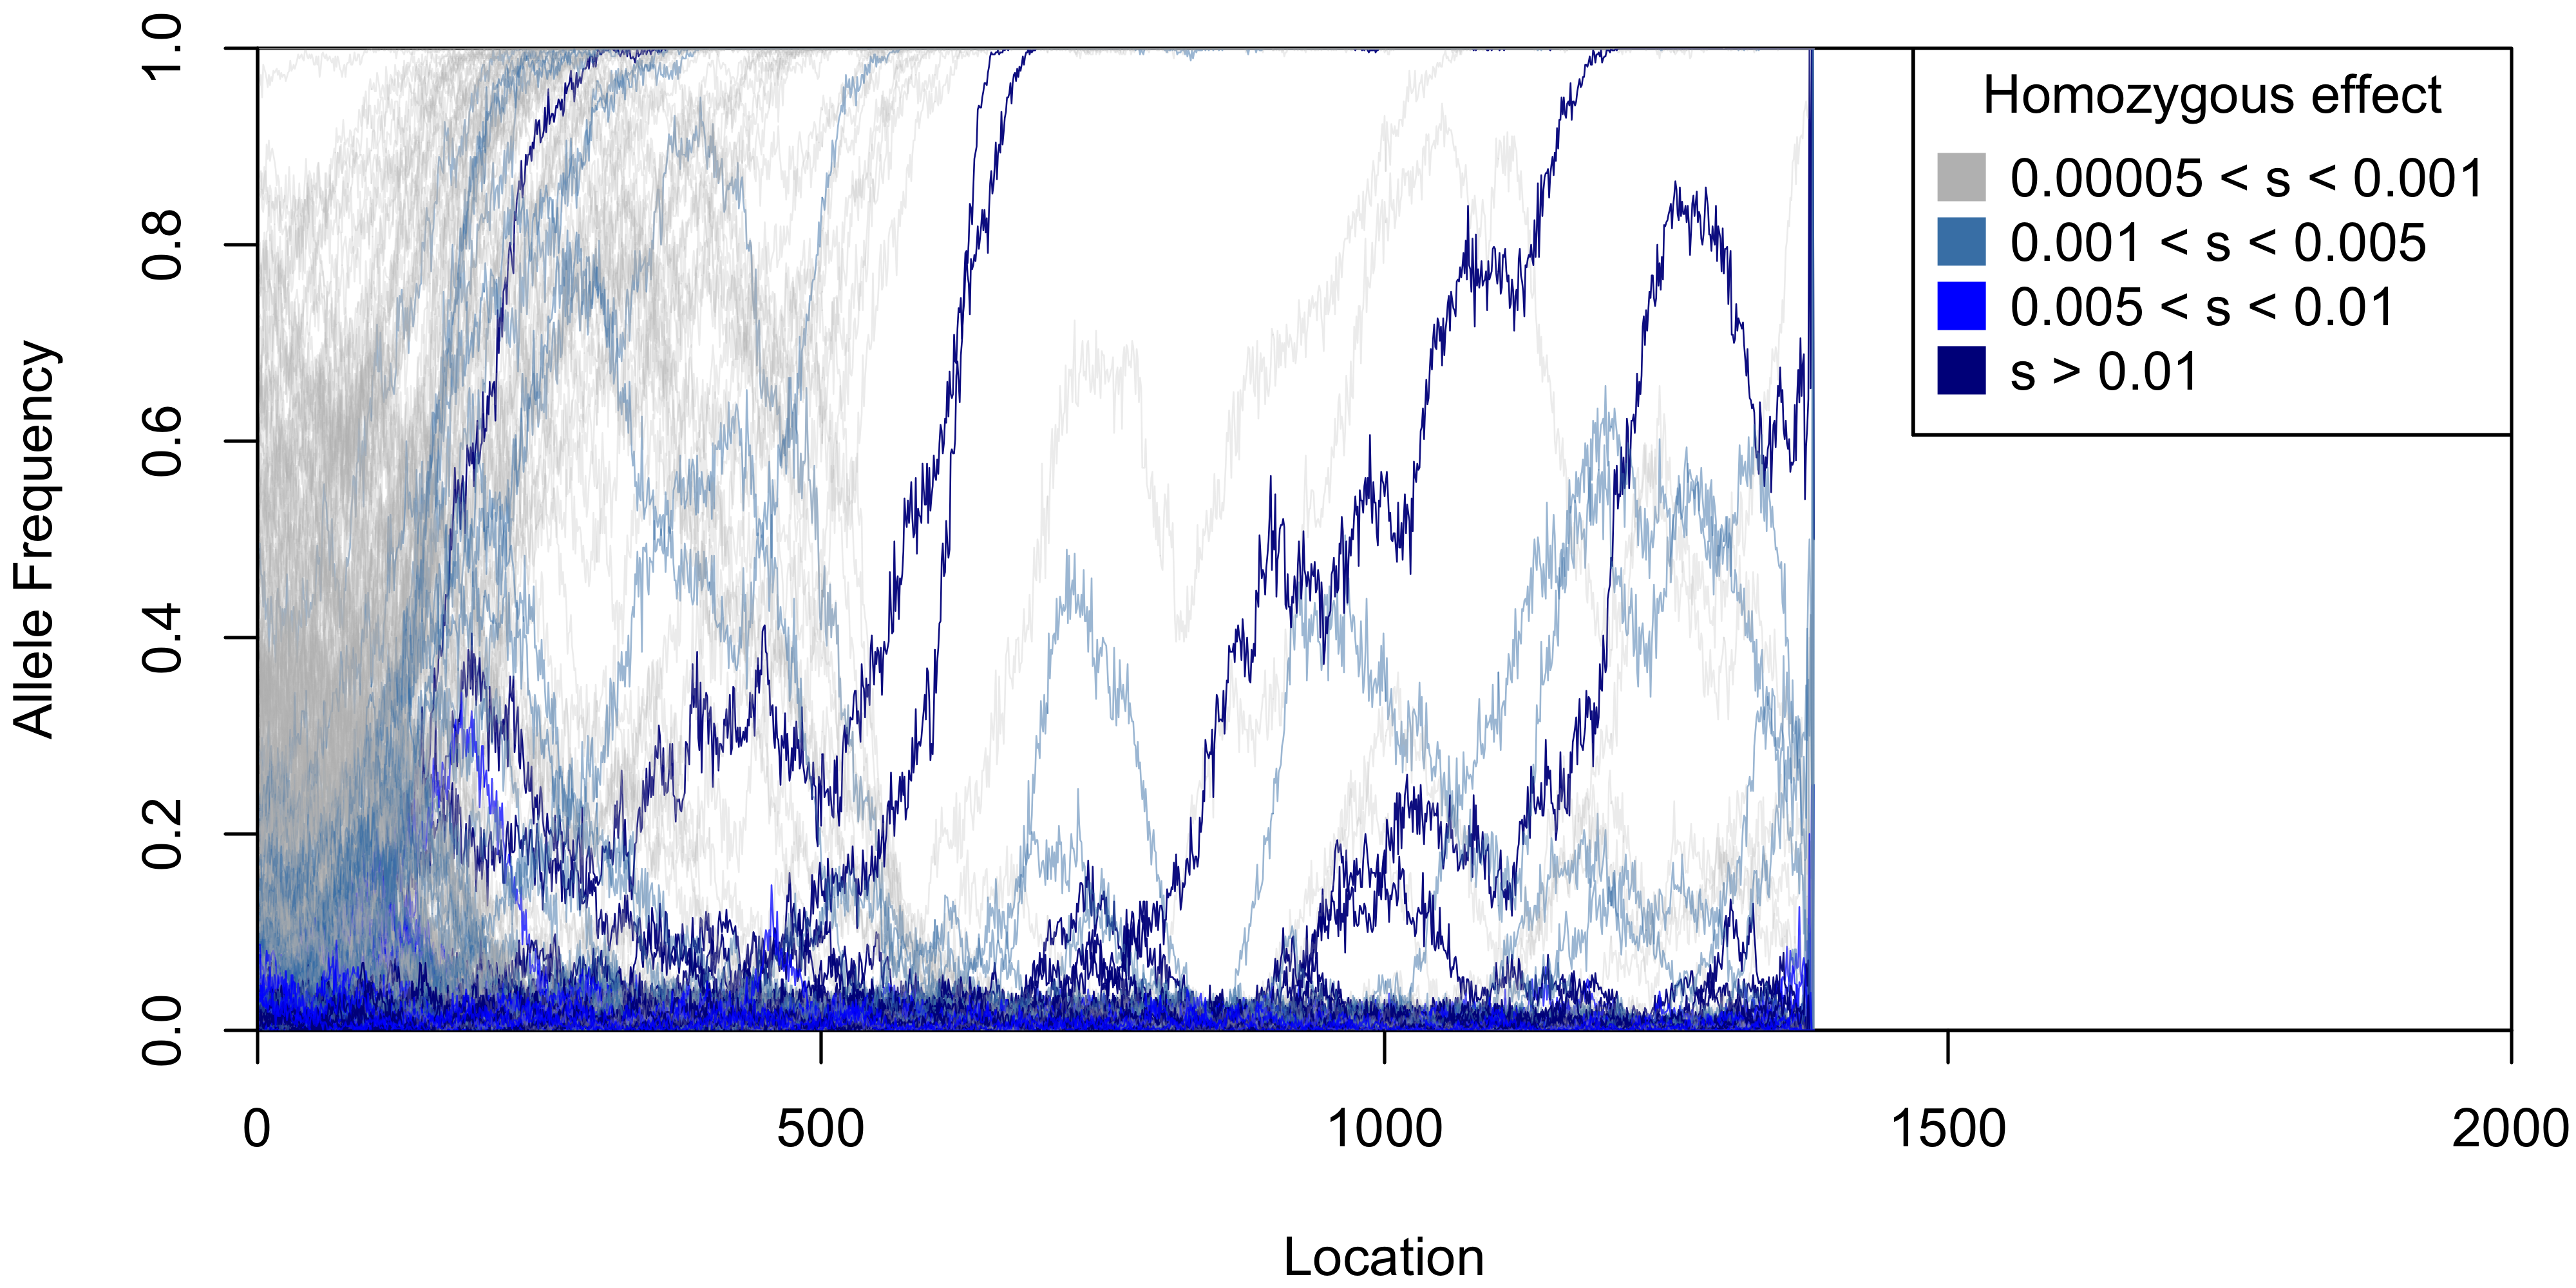
\includegraphics[width=0.9\linewidth]{Figures/example_allfreqs.png}}
\caption[~- Deleterious allele frequencies across the landscape.]{Deleterious allele frequencies across the landscape, by homozygous effect size, \emph{s}. This example is at 250 generations after burn-in for the case of a leptokurtic dispersal kernel, with $U_D = 0.1$ and $b = 0$. This example was not randomly chosen, but selected to show that large effect loci can locally fix under these conditions. The locus indicated by the thickest black line has an effect size of $0.0898$.}
\label{fig:allfreqs}
\end{figure}

% recovery rates in suppmat







%% add mike's point to discussion - in addition to the quanti trait redicing fitness and slowing expansion therefore reducing load, the same is true for more delet loci, i.e. load calcualted from one delet mut and multiplied up to more would overestimate the actual realized load

\section{Discussion}


%broadly start discussion for where our study fits into the literature of this field
%why no range limits are found
%compare to polechova and barton 2015
%could bring in relation to bridle et al 2010

Range expansions are unique demographic events that lead to an interesting suite of population genetic processes. These processes have been widely studied, yet the combination of both a heterogeneous environmental gradient and expansion load from deleterious mutations that can contribute to expansion load has not previously been investigated. Previous theoretical studies focusing independently on either the expansion load or adaptation along an environmental gradients predicted reduced fitness at the range edge. We find that these factors interact, so that the load at the expanding range edge is not as great as would be expected by a simple combination of the two. Both expansion load and local maladaptation to an environmental gradient reduce fitness at the range edge, but the mechanism of fitness reduction is important in the process of range expansion. Whether fitness is reduced due to local maladaptation or due to expansion load impacts the rate of range expansion, and therefore the rate of evolutionary rescue and thus the load that accumulates during expansion. This interaction is important for predicting the dynamics of modern range expansions due to natural phenomena or human-induced climate change. 

Our results corroborate previous studies, showing that expansion load accumulates at expanding range edges. Even though our simulation design differs from previous models investigating expansion load, we still find substantial load accumulating throughout the course of range expansion. The presence of hard versus soft selection can change the amount of expansion load accumulated \citep{Peischl:2013, Peischl:2015}, as can one- versus two-dimensional landscape models \citep{Peischl:2013}. Several other differences such as a range of mutational effects for deleterious alleles and continuous dispersal rather than a stepping-stone model might also contribute to the amount of expansion load.

%%We find an interesting interaction between migration load arising from an environmental gradient and expansion load arising from deleterious mutations in our simulations. The greatest expansion load ($39\%$) occurred in the absence of an environmental gradient. Rather than combining multiplicatively to further reduce fitness in edge populations, these factors instead interact to create a total load at the range edge that is not as bad as would be predicted. Steeper environmental gradients reduce expansion load, and higher deleterious mutation rates increase local adaptation to the environment. This effect would likewise have implications for 1-locus models of expansion load whereby it would be incorrect to assume an additive buildup of load when introducing more loci to a model.

%%We attribute this interaction to evolutionary rescue of one fitness component, allowed by the slower range expansion due to load in the other. Expansion across an environmental gradient is more difficult than in a homogeneous environment because local adaptation is impeded by the influx of maladaptive alleles from migrants \citep{Kirkpatrick:1997, Barton:2001, Polechova:2015}. This migration load alone can particularly reduce fitness at the range edge due to asymmetric migration from central populations \citep{Kirkpatrick:1997}. As the gradient steepens and increases the difficulty of local adaptation, fitness at the expanding edge decreases and expansion slows. This slower rate of expansion is key to the alleviation of expansion load because it provides increased time for evolutionary rescue and recovery from expansion load. When expansion is slowed, more migrants can reach the range edge, and population sizes can recover more quickly.

%%The fact that increasing deleterious mutations alone does not reduce expansion speed nearly as much as creating a steep environmental gradient explains the mechanism of the interaction of these two factors and emphasizes their significance. Expansion load that any given individual has accumulated would be equivalently detrimental to that individual's fitness regardless of where it existed on the landscape. The same is not true for the migration load that an individual might experience at the range edge. Maladaptation to the environmental gradient is changed if an individual is transplanted to a different location on the landscape. The population's survival is determined by total fitness, but the components of this fitness become meaningful when each changes the other. In our scenarios, increasing expansion load reduces total fitness at the range edge, therefore to survive and even exist, individuals must be more locally adapted. Successful expansion across a steep environmental gradient thus requires greater local adaptation than is otherwise needed in the absence of expansion load.

Our main result is that expansion load and the load due to local maladaptation interact. Local maladaptation at the range edge is not as severe in the presence of expansion load; and even more strongly, expansion load is not as severe in the presence of a strong environmental gradient causing local maladaptation. We believe that the dominant reasons differ for these two patterns of interaction. 

First, let us consider the improvement in the local adaptation at the range margin in the presence of expansion load. In order for a population to expand, the individuals at the expanding front must have an absolute fitness greater than one, on average. This means that a range margin will occur where absolute fitness drops below one. As a consequence, when there is greater load in one component of fitness, such as that caused by deleterious mutations across the genome, the population will not persist unless other fitness components are large enough to allow sufficient absolute fitness. Therefore, when expansion load is greatest, as occurs at the range edge, the fitness due to local adaptation must be higher in order for the population to have a large enough fitness to even exist. Note that this improvement in local adaptation is more a case of expansion load eliminating maladapted populations at the expanding front rather than a reduction in load. As a result, greater adaptation in the quantitative trait is found in the presence of expansion load.
%%This effect would likewise have implications for 1-locus models of expansion load whereby it would be incorrect to assume an additive buildup of load when introducing more loci to a model.

On the other hand, we also observe that expansion load can be greatly reduced in the presence of local maladaptation. In this case, we believe that there is an additional factor explaining this interaction.  In the absence of an environmental gradient, where the greatest expansion load accumulated ($39\%$), range expansion is mainly limited by dispersal ability. However, with local maladaptation caused by an environmental gradient, expansion is further slowed by the need for colonizing populations to adapt to the novel local environment. In fact, range expansion is slowed considerably more by a changing selective environment than by a high frequency of uniformly deleterious alleles (See figure \ref{fig:fitspeed}). As a result, the local maladaptation caused by a heterogeneous environment causes the rate of range expansion to slow substantially (Figure \ref{fig:speed}), which allows more time for evolutionary rescue of marginal populations. As range expansion slows, selection has more opportunity to reduce the frequency of deleterious alleles at the edge. Moreover, with slower expansion, high fitness alleles from the center of the range have more time to disperse toward the edge restoring genetic diversity at sites locally fixed for deleterious alleles by previous drift, and back mutation also has more time to generate beneficial diversity. In general, slower expansion ameliorates the conditions necessary for high expansion load at the range margin. Therefore, the local maladaptation caused by heterogeneous environments can reduce expansion load by slowing the rate of range expansion.

The mechanism altering expansion speed is a vital part of the process for these interactions to occur. When expansion is not slowed by the need to locally adapt and instead only by dispersal limitations, there is no expectation for a faster expansion to contribute to increased load. This explains the lack of further fitness reductions from increased expansion speed in our simulations with long distance dispersal. Instead, local adaptation at the edge was slightly reduced and expansion load less severe than in the Gaussian dispersal case, suggesting that this difference in dispersal models led to only slightly different amounts of expansion load accumulating given the different amount of connectivity between the core and edge. %%\citet{Fayard:2009} found that surfing was reduced in cases of long distance dispersal, substantiating this result. (\color{red} I think given our new interpretation of the results, Fayard no longer applies - will remove that part unless you think otherwise?\color{black})

Expansion load is attributed to the reduced efficacy of selection during expansion allowing detrimental mutations to accumulate, a result our study supports. The effect sizes of mutations underlying expansion load have important empirical implications, as many studies today aim to understand expansion load in humans after expansion out of Africa \citep{Henn:2015,Henn:2015b, Lohmueller:2014, Lohmueller:2014b, Gravel:2016}. Whether expansion load exists but is difficult to detect has been debated, and a full understanding of the selection coefficients across human (or other) genomes is lacking \citep{Hancock:2011, Henn:2015, Henn:2015b, Lohmueller:2014, Simons:2014}. We find an interesting difference in the make-up of expansion load between our two simulated cases of genome-wide deleterious mutation rates. While deleterious alleles of moderate and large effect are relatively rare, we find that they are responsible for the majority of expansion load. These alleles, which would otherwise tend to be purged or kept at low frequency by purifying selection, are able to increase in frequency on the expanding wave front. Interestingly, we find that in cases exhibiting faster range expansion, a larger proportion of expansion load comes from alleles of moderate and large effect, as purifying selection has less time to oppose the rise in frequency of strongly deleterious alleles.


\subsection*{Implications, Caveats, and Future Directions}

%% come back to this para after figure out speed implications
Our finding that local maladaptation interacts with expansion load has broad evolutionary and ecological implications, including studies of natural range expansions under climate change, invasive species, and conservation efforts \citep{Hunter:1994}. For example, highly invasive species are known for their rapid rate of spread (e.g., cane toads in Australia \citealt{Phillips:2006}), providing interesting opportunities to examine if and how these species accumulate expansion load. Conservation efforts that aim to reintroduce genetic diversity through assisted migration would clearly benefit edge populations in terms of reducing expansion load, but potential disruption to local adaptation is also a concern \citep{Aitken:2013}. Finally, both expansion load and migration load are likely to affect climate-change induced range shifts. Rapid climate change would necessitate fast range expansion. Therefore, expansion load may be increased and local adaptation decreased, leaving struggling populations subject to stochastic extinction events. If the speed of climate change is not too fast, however, populations adapting as they move over space may reduce any potential impacts of expansion load. 

There are several biological features of organisms and their environments that we did not consider in our simulations due to the vast computational resources already required, but these merit future investigation. Our simulations allowed for individuals to self-fertilize when mates were limited, but this is not possible in many species. The inability to self-fertilize could slow range expansions, leading to a reduction in the expansion load. Other effects can similarly reduce fitness in small edge populations. Allee effects \citep{Taylor:2005} or aggregating dispersal behavior that discourages colonization of empty habitat \citep{Altwegg:2013} would slow expansion, as might dispersal barriers or increased encounters with antagonistic species (e.g. competitors, pathogens) \citep{Case:2005, Kubisch:2013}. It would be interesting to consider species with overlapping generations, where previously established individuals may block immigration into patches at carrying capacity (i.e. a priority effect, \citealt{Atkins:2010}). Priority effects could slow replacement of initial colonizers at the range edge, impeding genetic rescue and increasing the persistence of expansion load away from the edge. Some factors which could speed expansion beyond rates seen in our model and lead to increased expansion load include greater long distance dispersal or increased fecundity. We found that simulations with fecundity halved ($3.5$ vs. $7$, data not shown) exhibited much less expansion load and higher fitness in edge populations. Thus, increasing fecundity allows populations to persist at lower mean fitness and thus accumulate more load. Finally, other factors could result in complex, less predictable effects.  Local adaptation likely involves multiple quantitative traits adapting over similar or different environmental gradients, with potentially complex interactions that merit future investigation.

A potentially key evolutionary component of range expansions not included in our model is the evolution of dispersal ability. Increased dispersal is always expected to evolve at expanding range margins \citep{Hargreaves:2014}. Interestingly, increased dispersal is expected theoretically and found empirically even during expansion across environmental gradients or with expansion load alone \citep{Henry:2015b}. However, increased dispersal also steepens the perceived slope of a given environmental gradient, which can eventually slow or even temporarily halt range expansion until edge populations evolve to overcome initial maladaptation (e.g. \citealt{Phillips:2012}). Therefore it is unclear how dispersal evolution would affect the results presented in the current study.


\subsection*{Conclusions}
% closing paragraph on broader implications

Our results support those of previous studies finding that expansion load via the surfing of deleterious alleles reduces fitness in expanding populations \citep{Peischl:2013, Peischl:2015, Peischl:2015b}. We show this under biologically realistic conditions, bolstering evidence that allele surfing may, indeed, cause expansion load in nature. Our results are also in agreement with those of previous studies showing that on an environmental gradient, migration load reduces fitness in expanding populations \citep{Kirkpatrick:1997, Bridle:2010, Polechova:2015}, though we did not see any cases of stable range limits as a result of local maladaptation nor expansion load. We highlight the mechanism of interaction between local maladaptation and expansion load. Local maladaptation feeds back to reduce the speed of expansion and thus allow for increased evolutionary rescue throughout range expansion. Finally, we demonstrate that faster range expansion leads to a larger contribution of moderate and large effect deleterious alleles to expansion load. These contributions significantly advance theory on the genetics of range expansion towards meaningful predictions and interpretations for studies of natural populations.




%%% Local Variables:
%%% TeX-master: "thesis"
%%% TeX-PDF-mode: t
%%% End:
